\section{Конструкторский раздел}

\subsection{Метод распознавания суицидальных паттернов поведения человека по текстовым сообщениям}

Метод распознавания суицидальных паттернов поведения человека по текстовым сообщениям включает в себя xранение и анализ сообщений пользователей -- для определения, является ли сообщение суицидальным, используется модель машинного обучения. В качестве обучающей выборки используется дополненный датасет размеченных сообщений из открытого доступа \cite{dataset}.

\subsection{Формат и метод сбора данных }

В качестве задействованных в анализе данных используются текстовые сообщения и их даты написания, так как представленная зависимость количества смертей от суицида в зависимости от года и месяца говорит о возможной корреляции месяца написания сообщения и его возможной интерпретации.

\textbf{Тут надо рассказать про бота, угу}

\subsection{Декомпозиция системы}

На рисунке \ref{img:useCase} представлена диаграмма вариантов использования системы.

\begin{figure}[H]
	\centering
	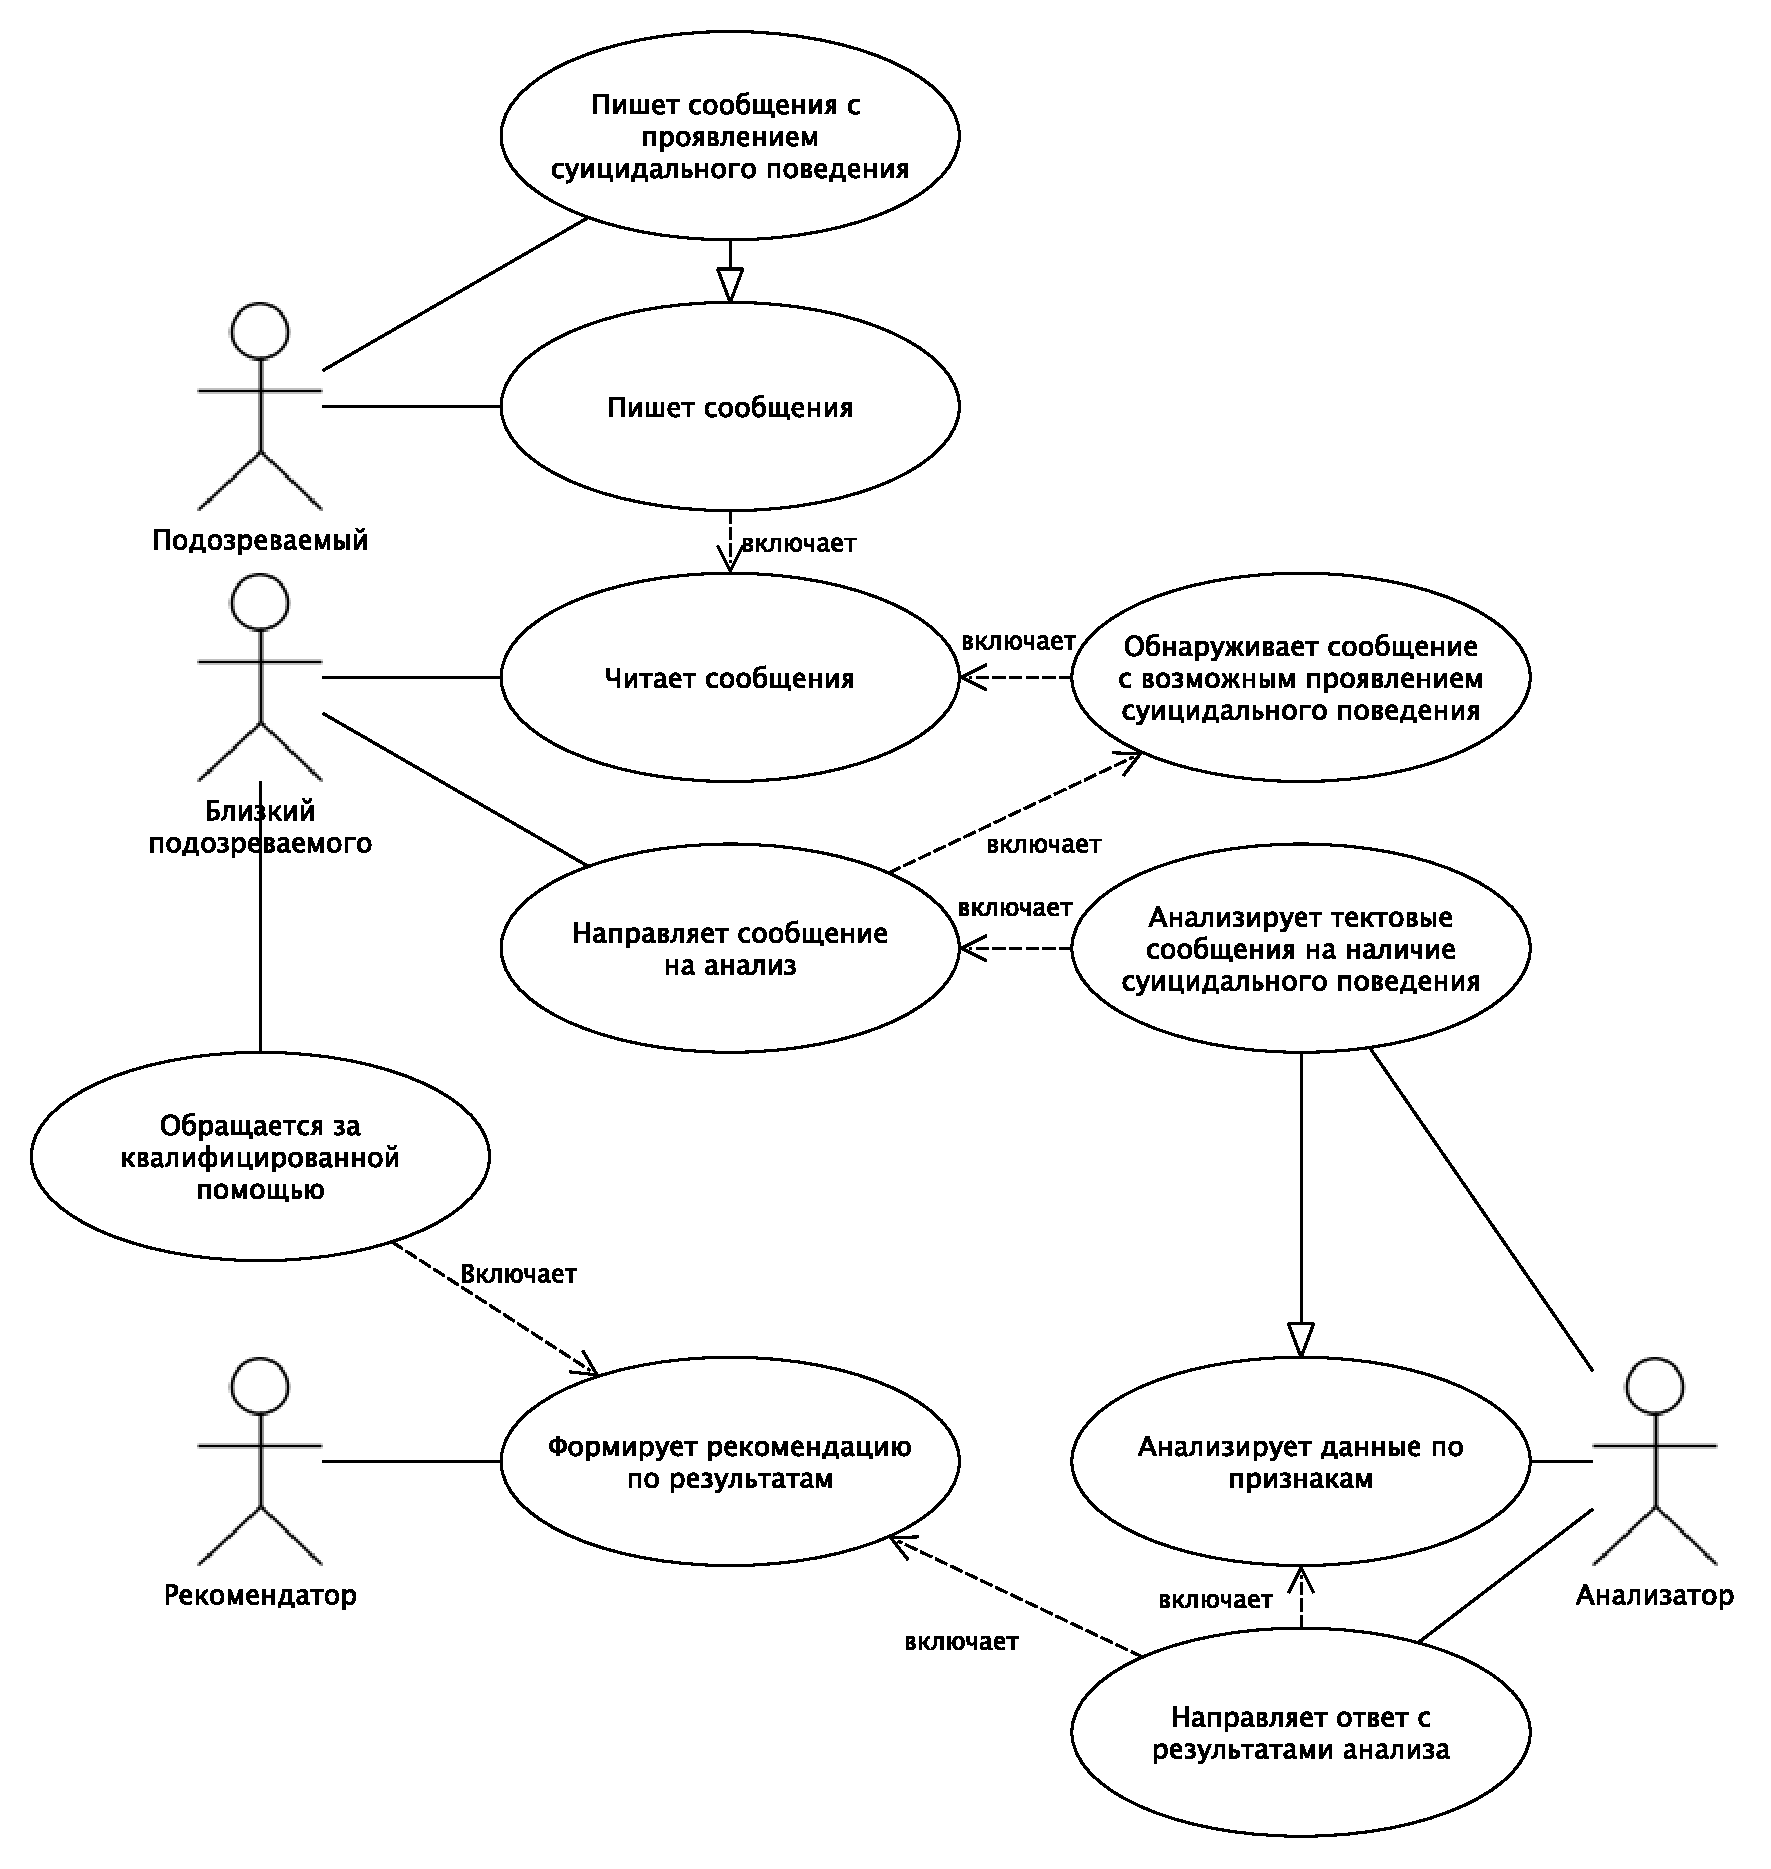
\includegraphics[width=\textwidth]{inc/useCase.pdf}
	\caption{ Диаграмма вариантов использования системы. }
	\label{img:useCase}
\end{figure}

\pagebreak